\PassOptionsToPackage{bookmarks=false}{hyperref} 
 \documentclass[conference]{IEEEtran}
\IEEEoverridecommandlockouts
% The preceding line is only needed to identify funding in the first footnote. If that is unneeded, please comment it out.
%\usepackage{cite}
\RequirePackage[utf8]{inputenc}     % UTF8 encoding
\RequirePackage[english]{babel}     % english language
\RequirePackage{microtype}          % improved kerning, layout
\RequirePackage{graphicx}           % graphics
\RequirePackage[caption=false,font=footnotesize]{subfig}
\RequirePackage[hidelinks, bookmarks=false]{hyperref}
\RequirePackage{caption}
%\RequirePackage[bottom]{footmisc}
\usepackage[hang,flushmargin]{footmisc}

\usepackage{setspace}
\setstretch{1.0}

%


% write PDF metadata
\makeatletter
\AtBeginDocument{
% set pdfoptions
\hypersetup{
     pdftitle={WoT-CI: Web of Things System Continuous Integration},
     pdfauthor={Muthuraman Chidambaram, Ege Korkan, Sebastian Steinhorst},
     pdfkeywords={Internet of Things, \ac{td}, CPS, Model-driven development, System Testing }% manual copy
   }
}
\makeatother
%pdfkeywords={IoT, WoT}

%\usepackage{amsmath,amssymb,amsfonts}
\usepackage{algorithm}
\usepackage{algorithmic}
\usepackage{textcomp}
%\usepackage{algpseudocode}
\graphicspath{ {images/} }
%\usepackage{text comp}
\usepackage{listings}
\usepackage[nolist,nohyperlinks]{acronym}
\usepackage{todonotes}
\presetkeys{todonotes}{inline}{}
\usepackage{amsthm}
\theoremstyle{definition}
\newtheorem{definition}{Definition}[section]
\def\BibTeX{{\rm B\kern-.05em{\sc i\kern-.025em b}\kern-.08em
    T\kern-.1667em\lower.7ex\hbox{E}\kern-.125emX}}
    

\usepackage{url}
\usepackage{xcolor}
\colorlet{punct}{red!60!black}
\definecolor{background}{HTML}{EEEEEE}
\definecolor{delim}{RGB}{20,105,176}
\colorlet{numb}{magenta!60!black}
\lstdefinelanguage{json}{
    basicstyle=\ttfamily\footnotesize,
    numbers=left,
    numberstyle=\scriptsize,
    stepnumber=1,
    numbersep=8pt,
    showstringspaces=false,
    breaklines=true,    
    backgroundcolor=\color{background},
    literate=
      {:}{{{\color{punct}{:}}}}{1}
      {,}{{{\color{punct}{,}}}}{1}
      {\{}{{{\color{delim}{\{}}}}{1}
      {\}}{{{\color{delim}{\}}}}}{1}
      {[}{{{\color{delim}{[}}}}{1}
      {]}{{{\color{delim}{]}}}}{1},
}
\lstdefinestyle{json}{
  float,
  floatplacement=t,
  %abovecaptionskip=-5pt,
  belowcaptionskip=-15pt,
  language=json, 
  float=h, 
  numbers=left, 
  numberstyle=\tiny, 
  stepnumber=1, 
  numbersep=1pt, 
  captionpos=b, 
  xleftmargin=1em,
  framexleftmargin=1em
}
\AtBeginDocument{
\captionsetup{font={footnotesize}}
\captionsetup[lstlisting]{belowskip=-100pt, aboveskip=6pt}  % no effect!
\captionsetup[figure]{belowskip=-10pt, aboveskip=6pt}
\captionsetup[table]{belowskip=-10pt, aboveskip=3pt}   
}
%\renewcommand{\baselinestretch}{1.52}
\begin{document}

\title{WoT-CI: Web of Things System Continuous Integration \\
}

\author{
  \IEEEauthorblockN{Muthuraman Chidambaram}
  \IEEEauthorblockA{
    \textit{Technical University of Munich (TUM)}\\
    \textit{Munich, Germany}\\
    \textit{muthuraman.chidambaram@tum.de}
  }
  \and
  \IEEEauthorblockN{Ege Korkan}
  \IEEEauthorblockA{ 
    \textit{Technical University of Munich (TUM)}\\
    \textit{Munich, Germany}\\
    \textit{ege.korkan@tum.de}
  }
  \and
  \IEEEauthorblockN{Sebastian Steinhorst}
  \IEEEauthorblockA{
    \textit{Technical University of Munich (TUM)}\\
    \textit{Munich, Germany}\\
    \textit{sebastian.steinhorst@tum.de}
  }
}

\maketitle
 


\begin{abstract}

  Number of Internet of Things (IoT) devices are growing exponentially with the development of the smart city, connected car and industry 4.0.
  % As of August 2019, there are 26 billion (and growing active) IoT devices in business and consumer space. 
  % But 42 billion connected IoT devices are required by the year 2025. 
  % We are supposed to produce 16 billion flawless connected devices in the next 5 years.
  As of 2019, there are 26.6 billion IoT devices. 
  But, the major drawback of the IoT ecosystem is its highly fragmented nature. 
  Even if infinite solutions are arising, most of them are incompatible and reflect the needs of particular use-cases and technologies. 
  The World Wide Web Consortium (W3C) Web of Things (WoT) is intended to enable interoperability across IoT platforms and application domains. 
  In the act of using WoT for deploying IoT platform, WoT has reduced a considerable amount of time for the IoT platform developers. 
  Though the platform deployment time is reduced by WoT, it is still a problem of the platform developers to make sure the IoT platform is working as per the requirements after individual device upgrades.  
  In this paper we introduce WoT-CI, a method that uses the principles of Continuous Integration (CI) in the context of WoT, by considering the WoT devices as contributors and WoT system as a single software project. We show that this system can reduce system integration effort while requiring no manual input from the developer, thereby, assuring that the WoT devices are functioning as per the requirement after any change to the hardware, software or network.


\end{abstract}

\begin{IEEEkeywords}
Internet of Things, Upgrade, Web of Things, System Testing
\end{IEEEkeywords}

\section{Introduction} \label{introduction}

\ac{iot} is a system of interrelated computing devices like smart home appliances, smart medical appliances and computer devices. 
Each device that is attached with a sensor and an actuator and can communicate via the Internet is an \ac{iot} device. 
The number of \ac{iot} devices is growing exponentially with the development of the Smart City, Connected Car and Industry 4.0. 
As of August 2019, there are 26 billion (and growing active) \ac{iot} devices in business and consumer space.
All these devices are built under different architecture and principles. 
\ac{iot} platform developers are supposed to interact with these devices in completely different methods due to its highly fragmented nature.  
% But, the major drawback of the \ac{iot} ecosystem is its highly fragmented nature. 
% Even if infinite solutions are arising, in both the consumer and business market, most of them are incompatible and reflect the needs of particular use-cases and technologies.
As a consequence, IoT system architects are forced to either use a single system (thus limiting the number of available devices) or to face several compatibility issues. 
Moreover, different standards cannot leverage the device to device concepts, as they will always require an adaptation element to ensure interoperability. \cite{fantacci2014short}


The \ac{w3c} \ac{wot} is intended to enable interoperability across \ac{iot} platforms and application domains. 
Overall, the goal of the \ac{wot} is to preserve and complement existing \ac{iot} standards and solutions. 
The \ac{w3c} \ac{wot} achieves interoperability through wider adoption of the Web principles, standardized device description via \ac{td} standards, metadata and semantic web technologies. 

A \ac{td} describes the metadata and interfaces of Things, where a Thing is an abstraction of a physical or virtual entity that provides interactions to and participates in the \ac{wot}. 
Thing Descriptions provide a set of interactions based on a small vocabulary that makes it possible both to integrate diverse devices and to allow diverse applications to interoperate. 
Thing Descriptions, by default, are encoded in a JSON format that also allows JSON-LD processing. 

\begin{figure}[t]
  \centerline{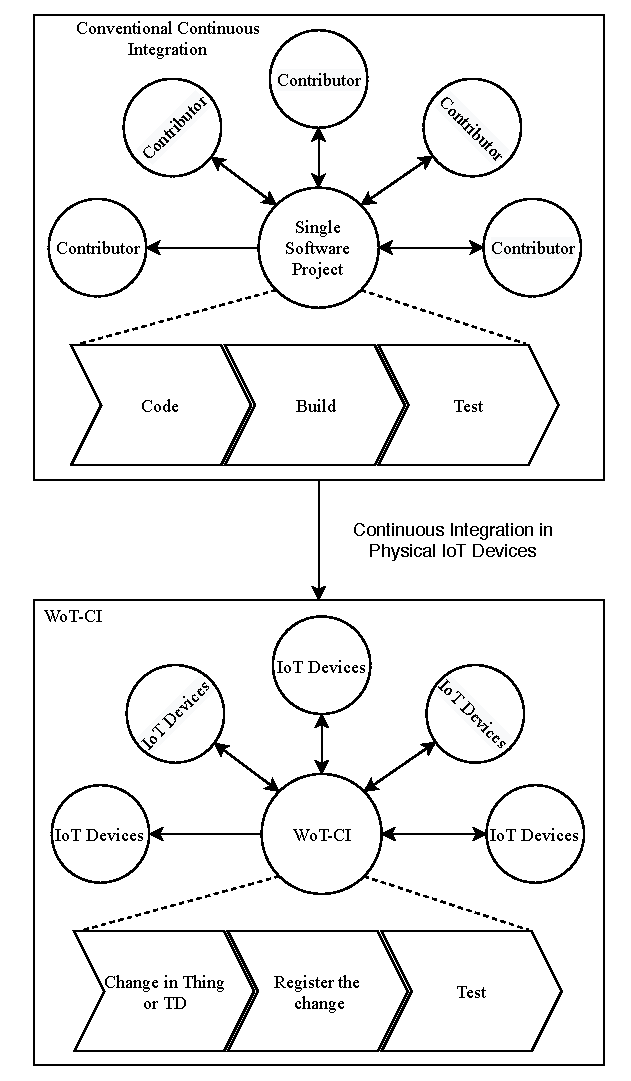
\includegraphics[scale=0.6]{iotSystem} }
  
  \caption{The figure describes the use of Continuous Integration in WoT-CI: The principles of Continuous Integration (CI) in the context of WoT, by considering the WoT devices as contributors and WoT system as a single software project}
  \label{fig:WoT-CI}
\end{figure}

\textbf{Problem. }\ac{wot} can be easily integrated into the \ac{iot} platforms to enable horizontal business cases and applications. 
Apart from that, utilization of the Web Technology reduces testing time and deployment of RESTful web services \cite{datta2018advances}.
Even though the platform deployment time is reduced by WoT, it is still a problem of the platform developers to make sure the IoT platform is working as per the requirement after any change to the hardware, software or network.

In the conventional software development, Continuous Integration (CI) is a software development practice where members of a team integrate their work frequently, usually each person integrates at least daily - leading to multiple integrations per day. 
Each integration is verified by an automated build (including test) to detect integration errors as quickly as possible. 
Many teams find that this approach leads to significantly reduced integration problems and allows a team to develop cohesive software more rapidly.\cite{fowler2006continuous}

\textbf{Contribution. }In this paper we introduce WoT-CI, a method that uses the principles of Continuous Integration (CI) in the context of WoT, by considering the WoT devices as contributors and WoT system as a single software project. 
Our contribution in this paper shows that this system can reduce system integration effort while requiring no manual input from the developer, thereby, assuring that the WoT devices are functioning as per the requirement after any change to the hardware, software or network. Refer figure: \ref{fig:WoT-CI}
% First, we describe the State of the art of Continuous Integration in \ac{wot}. 
% Second, we state the methods and materials used in solving the problem. 
% Third, we explain our approach used in our system. 
% Fourth, we share the results of our work. Finally, we state the future work in the field and give our conclusion to the solution.

\section{State of the Art}

Testing an \ac{iot} device is significantly different from testing a typical hosted software as the \ac{iot} devices are resource constrained devices \cite{bormann2014terminology}. 
Since end-to-end testing in \ac{iot} system involves physical devices, a complete automation testing suite usually cannot be deployed on the IoT device. 
IoT software components are strongly coupled with the hardware \cite{rosenkranz2015distributed}.

As stated earlier in this paper, each Thing in the \ac{wot} ecosystem has a \ac{td}which describes the metadata and interfaces of Things. 
Thereby, this \ac{td} a JSON object is further used for testing the Things in \ac{wot} ecosystem. 
The testbench tool can test a \ac{wot} Thing by executing interactions automatically, based on its \ac{td}. 
Each interaction is executed based on the Representational State Transfer (REST) and Publisher Subscriber Model. 
But testbench is a tool which can test \ac{td} of a Thing, when the \ac{td} is provided to the tool.

Most commonly, \ac{iot} device software is tested with the help of simulators and emulators. 
The approach in \cite{karlesky2007mocking} is to test the software developed for embedded devices that are resource constrained. 
There are multiple benefits while using an emulator or simulator, hardware and software can be developed parallelly as there is no dependency hardware for testing the software. 
An end to end test setup can be developed with the help of Continuous Integration and Continuous Development (CI/CD) tools like Jenkins, CircleCI and more. 
Therefore, this setup will be much faster than the normal testing setup. 
But the problem with the emulator is that, it is impossible with the current technology to emulate all possible sensors and actuators in the \ac{iot} device market. 
This problem is an extensive constraint for the developers. 

In \cite{osterlind2006cross} Cooja Simulator, a cross-layer Java-based Wireless Sensor Network (WSN) simulator distributed with Contiki. 
It allows the simulation of different levels from physical to application layer, and also allows the emulation of the hardware of a set of sensor nodes. 
This system can simulate wireless communication medium and perform a complete white-box testing. 
This approach also shares the benefits and drawbacks of the approach of \cite{karlesky2007mocking}.
 
\cite{okola2010unit} presents a new unit testing framework that addresses this concern by defining tests as a single Python script that executes on the PC. 
This script automatically generates test programs, coordinates the inputs, and collects outputs from all nodes in the network. 
This approach allows validation of distributed state, while simultaneously reducing the amount of code needed to define a unit test. 
But this tool requires to know each variable and function, while requiring one line of code for each function or variable. 
Therefore, this tool adds manual work to the developer. 

\cite{woehrle2007increasing} presents essential features of a framework for testing a broad range of WSN applications. 
Here the Self-testing is achieved by explicitly specifying the inputs and the expected outputs of the software under test in an executable format. 
This allows for partial automation of the test procedure. 
Automated testing promotes frequent execution of the tests and enables the designer to continuously compare the implementation’s behavior with the specification in multiple platforms. 
But still the developer has to explicitly specify the inputs and outputs for Software Under Test (SUT).

Though the approaches above are satisfying most of our problem case, we don’t have a complete solution for getting rid human intervention to assure that the \ac{iot} devices are functioning as per the requirement after any change to the hardware, software or network. 
The methods which rely mostly on either emulators or simulators are elegant in terms of the offered test workflow. 
However, they are also difficult to implement for projects which support many different device types \cite{rosenkranz2015distributed}.

\section{A Comprehensive WOT-CI Test System Architecture}

We propose a test system architecture for \ac{wot} software development that is not only scalable in the number of supported device types, but also in the number of test scenarios. 
It allows any device that is built with the support of \ac{wot} \ac{td}.  
Our system is designed to perform a complete black box testing on all \ac{wot} devices in the \ac{wot} ecosystem
In this section, we initially give an overview of the architecture, then justify the design decision and finally discuss their results.

\begin{figure}[t]
  \centerline{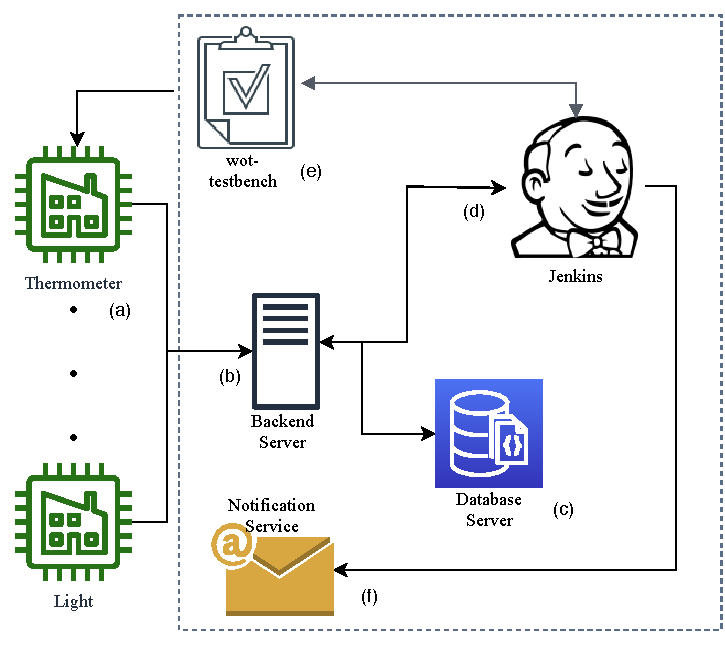
\includegraphics[scale=0.7]{arch} }
  \caption{The figure above depicts the architectural overview of WoT-CI}
  \label{fig:Architecture}
\end{figure}

\subsection{Architectural Overview: }
Our architecture consists of \ac{wot} Things, backend server, database server, automation server, testing framework and a notification service. 
A test platform can be one or more \ac{wot} devices connected to the Internet and the devices can talk in multiple protocols as the test framework. 

The \ac{wot} Thing (Fig. \ref{fig:Architecture}(a)) is any device that has a set of sensors and actuators and can connect to internet via its interface. 
Most importantly the Thing must have \ac{wot} \ac{td}. 
The task of the \ac{wot} Thing is to register their \ac{td} with WoT TD standards to the Web Server. 
Things are expected to send their \ac{td}, whenever there is software or hardware update on the Thing or on a failover scenario or during network change.
Manual registration of \ac{td} is also possible.
A Thing can also communicate with other devices during testing to perform integration testing.

The backend server (Fig. \ref{fig:Architecture}(b)) is a programmatic interface consisting of one or more publicly exposed endpoints to a defined request–response message system. 
The backend server is additionally assigned to trigger the automation server whenever there is a new \ac{td} added to the database and store the result from automation server to database.
In our system we have exposed end points to perform all database operations like read, write, update or delete. 
The task of the backend server is to process the request and perform the corresponding action in the database and send response to the Things or to a API Client.

The database server (Fig. \ref{fig:Architecture}(c)), adopt any database as a backend to store and retrieve.  
In our system, the database server has two models or tables, first to store the \ac{td} and second to store the credentials of automation server. 
The task of the database server is to perform the actions sent by requests from backend server and return a response with success or failure. 
Additionally, the database server is supposed to maintain the last five versions of \ac{td} and consecutive two versions should not have the same \ac{td}. 

The automation server (Fig. \ref{fig:Architecture}(d)) is a tool which enables developers around the world to reliably build, test, and deploy their software. 
In our architecture we need an automation server which does not require a codebase to perform automation. 
As we are using the concept of continuous integration to trigger a build for an update on database, our automation server must be capable of sending the test results to the users. 
The task of the automation server is to 
\begin{itemize}
  \item Clone or download the Web server and test framework repositories.
  \item Build both the repositories.
  \item Start the build to fetch all the Thing Descriptions from the database with the help of Web server.
  \item Run all the Thing Descriptions against the test framework.
  \item Send the test results to the developer.
\end{itemize}

The test framework (Fig. \ref{fig:Architecture}(e)) is a set of guidelines or rules used for creating and designing test cases. 
In our architecture the test framework must be based on \ac{td} from \ac{w3c} \ac{wot}. 
The task of the test framework is to test the Thing Descriptions in a sequential manner. 
A \ac{td} should represent capabilities of a device. 
This implies that if a device supports the interactions that a client can execute based on the device's \ac{td}, it doesn't comply to its own \ac{td}. 
The test framework must generate fake data for each variable in the \ac{td} and send, read request and write request to the Thing and validate the user access rights and additionally send command to all actions in the \ac{td} via IoT protocols and validate the response. 

The notification service (Fig. \ref{fig:Architecture}(e)) is a any application that enables configuring one or more contact identities to receive, read, compose and share information with interested groups. 
In our architecture, we require a client which can collaborate with our automation server. 
The task of the notification service is to fetch the result and log from test framework and send it to developers and return the status of the response client send function to the automation server. 
A response is supposed to be send for every build irrespective of build success or failure.

\subsection{Architectural Elements}

The Architectural overview presented earlier is implemented with the following elements.

\subsubsection{Things:}

The \ac{wot} Things considered are developed using different protocols such as HTTP, MQTT and CoAP and are programmed differently\footnote{Source code for these devices are available here: https://github.com/tum-esi/wot-sys.git}. 
% in this architecture is developed with code guidelines of WoT-SYS tum-esi in github. 
% Wot-SYS is a project that contains the source code, description, guides etc. of the \ac{wot} System that will be used by students of Embedded Systems and Internet of Things (ESI) in Technical University of Munich.

\subsubsection{Backend Server:}
  
The backend express server in this architecture is developed with NodeJS programming language. 
\begin{itemize}
  \item The Web Server holds function to get and post \ac{td} from/to the database.
  \item The Web server is additionally configured to trigger automation server, whenever a \ac{td} is added to the database.
  \item The Web server is designed to store five versions of \ac{td} from the same ID tag with a feature of not holding consecutive \ac{td} with same value.
\end{itemize} 

NodeJS is used for the asynchronous call feature. 
Therefore, with the asynchronous feature NodeJS is lighter and faster than other scripting languages.

\begin{figure}[t]
  \centerline{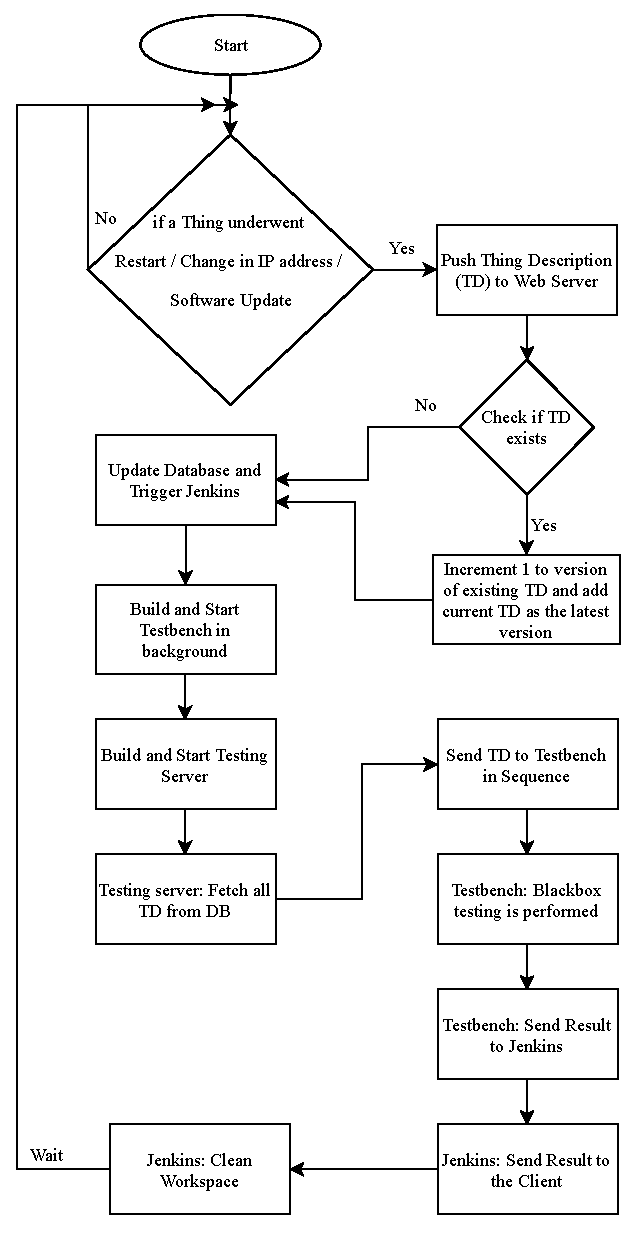
\includegraphics[scale=0.9]{SystemFlowChart} }
  
  \caption{The flowchart above illustrates the flow of the WoT-CI, starting from the system inspecting for a change on Thing to testing new or updated TD and notifying the results of the Thing to the User}
  \label{fig:Algorithm}
\end{figure}

\subsubsection{Automation Server:}

Jenkins is used as an automation server. 
The open source automation server, Jenkins provides hundreds of plugins to support building, deploying and automating any project. 
Major reason for using Jenkins is to use the concept of freestyle project in Jenkins, wherein we need not link the automation server to repository. 
Since Jenkins is a highly customizable opensource tool, we are using Jenkins to perform the Continuous integration part.  
Jenkins, in addition to the continuous integration part, it can collaborate with an response client and send out responses. 
Jenkins runs the build on any machine. 
In our architecture, Jenkins is configured to run on the same machine and to delete the workspace before every built.

\subsubsection{MongoDB:}

MongoDB is widely used across various web applications as the primary data store. 
One of the most popular web development stacks, the MEAN stack employs MongoDB as the data store (MEAN stands for MongoDB, ExpressJS, AngularJS, and NodeJS). 
MongoDB is a document database, which means it stores data in JSON-like documents. 
In our architecture, MongoDB is configured with a database with two collections, 

\begin{itemize}
  \item First collection is for storing the Jenkins credentials
  \item Second collection is for storing the \ac{td}
\end{itemize}

\subsubsection{Test Framework: }

In this architecture, we are using a publicly available wot-testbench\footnote{wot-testbench tool is available in https://github.com/tum-esi/testbench.git} tool from tum-esi in github.  
Test bench tests whether: 
\begin{itemize}
\item Every interaction written in the TD can be executed
\item Writable properties are indeed writable
\item Each interaction returns the described data type\footnote{DataSchema of TD Specification}. 
\end{itemize}
The testbench generates fake data for each variable in the \ac{td} and send read request and write request to the Thing and validate the user access rights and additionally send command to all actions in the \ac{td} and validate the response.

\subsubsection{Response Client:}

In this architecture Google mail is used as an response client as it enables us to generate app password. 
An App Password is a 16-digit passcode that gives a non-Google app or device permission to access your Google Account. 
App Passwords can only be used with accounts that have 2-Step Verification turned on.

\section{Approach}

The approach illustrated in the fig. \ref{fig:Algorithm} is explained below.

\subsection{Generation of \ac{td}:}
  
A \ac{wot} Thing is supposed to register their own \ac{td} to Web API Server on three different occasions:

\begin{itemize}
\item When the Thing is hard or soft restarted.
\item When the Thing is assigned with a new Internet Protocol Address.
\item When there is software or hardware update on the Thing.
\item When a \ac{td} is updated manually.
\end{itemize}

\subsection{Update \ac{td} to Database and Trigger Jenkins Build:}
  
Once the Web API Server receives the \ac{td}.
\begin{itemize}
  \item The \ac{td} “ID” received is compared against the existing \ac{td} in the database.
  \item If there are no similar existing \ac{td}, 
    \subitem then a version tag is added in addition to \ac{td} and the \ac{td} saved to the database.
  \item Response from the database is forwarded to the user.
  \item If there are few existing similar Thing Descriptions available in the database, 
    \subitem then the received \ac{td} is compared with the existing latest version of \ac{td} for exact match.
  \item If there is an exact match,
    \subitem then the user is responded, stating that the \ac{td} sent is similar to the previous one and the \ac{td} is not updated in the database.
  \item If there is no exact match,
    \subitem then the version number is updated for the existing Thing Descriptions and the received \ac{td} is saved as the latest \ac{td} to the database\footnote{Since we maintain only the last five versions of \ac{td}, the oldest version is deleted from database if we have five versions for a particular \ac{td} ID.}.
  \item When the database is updated with a new \ac{td}, Jenkins build is called to perform the Continuous Integration concept.
\end{itemize}

\subsection{Jenkins Build:}
  
On receiving the build trigger for an item, Jenkins is configured to clean up the previous build log and perform the following task:

\begin{itemize}
\item Clone the testbench repository from tum-esi in github, build the repository and start the testbench tool.
\item Clone the wot-ci repository from tum-esi in github, build the repository and start the testing server.
\item Send the result of the test to the users via email.
\end{itemize}

The task of testing server is to fetch all the latest \ac{td} from the database and test it by running it against the testbench.
The results and logs and accumulated from the Jenkins workspace and sent to the interested user or user group.

\subsection{Testing Framework:}

Testbench started by Jenkins build will be waiting for a \ac{td}. 
Once it receives a \ac{td}, fake data and calls are generated by testbench and waits for an API call from the testing server, once the testing server send an API call, the call is executed and the \ac{td} is tested based on the user requirement.
Testbench can be used to perform unit test as well as integration test. 
The fasttest action in the testbench tool is used for the integration test. 
As a result of this function a test report is generated and returned to the testing server.

\section{Conclusion}

The combination of resource constrained platform and the highly fragmented nature has made \ac{iot} system testing a challenge.
Unfortunately, we are unable to achieve the expectations with the emulators.
In this paper, we analyzed the challenges of system testing in \ac{iot} devices and presented a test system architecture to perform a automated system test for \ac{iot} devices.
The presented architecture is supposed to be used for blackbox system testing for \ac{w3c} \ac{wot} ecosystem. 
In this paper we introduce WoT-CI, a method that uses the principles of Continuous Integration (CI) in the context of \ac{wot}, by considering the \ac{wot} devices as contributors and \ac{wot} system as a single software project. We show that this system can reduce system integration effort while requiring no manual input from the developer, thereby, assuring that the \ac{wot} devices are functioning as per the requirement after any change to the hardware, software or network.
% Additionally, it takes only one minute and thirty seconds for fifteen device in a isolated ecosystem under a Local Area Network (LAN).
% Furthermore, we have overcome the interoperability problem with the support of \ac{wot} \ac{td}.

\textbf{Future work.} Though we have achieved continuous integration in the \ac{wot} ecosystem, it is still not equivalent to end to end automation.
A manual work is required to deploy the software into microcontrollers. 
Since every microcontroller cannot be accessed through telnet or secure shell, it is still a research topic to build an application to deploy the microcontroller software into microcontroller without physical contact.  
This problem is an extensive constraint for the developers.
One approach we are considering is to use terraform to do deploy the software into microcontrollers to complete the full automation, but many \ac{iot} devices are not accessible via secure shell or telnet connections.  



\begin{acronym}[ECU]
\acro{iot}[IoT]{Internet of Things}
\acro{td}[TD]{Thing Description}
\acro{w3c}[W3C]{World Wide Web Consortium}
\acro{wot}[WoT]{Web of Things}
\acro{uri}[URI]{Uniform Resource Identifier}
\end{acronym}

%\renewcommand{\baselinestretch}{1.00}
\setstretch{1.0}
\bibliographystyle{IEEEtran}
\bibliography{bibliography}

%\hyphenation{cryp-to-graphy}


\end{document}
